% Work-MAT -- 2. rocnik, hodina 07. Mocninne funkce se sudym a lichym exponentem.
\documentclass[11pt,a4paper]{article}
\input{../../sablony/pripravy/priprava.sty}
\usepackage{tikz}
\usetikzlibrary{arrows.meta}
\nastavPripravu{2. ročník}{Mocninné funkce}{07}{Mocninné funkce I: kladné exponenty}
\begin{document}
\poznamka{Navazujeme na inverze, ale dnes je cílem přehled rodiny $x^n$. Orientačně 5 min motivace, 12 min sudé exponenty, 10 min liché exponenty, 12 min příklady a samostatná práce, 6 min shrnutí. Znalosti 1. ročníku (parabola, prostota, sudost) aktivně využívej.}

\blok{Jedna rodina funkcí, různé tvary grafu}
Známe již přímku $y=x$, parabolu $y=x^2$ i graf $y=x^3$. Všechny patří do rodiny mocninných funkcí. Jejich tvar a vlastnosti závisí především na tom, zda je exponent \emph{sudý} nebo \emph{lichý}.

\begin{definiceBox}[title={Definice - Mocninná funkce s kladným celočíselným exponentem}]
Pro celé číslo $n\ge1$ je \textbf{mocninná funkce} funkce daná předpisem $f(x)=x^n$ pro všechna $x\in\mathbb R$.
\end{definiceBox}

\begin{center}
\begin{minipage}{.47\linewidth}\centering
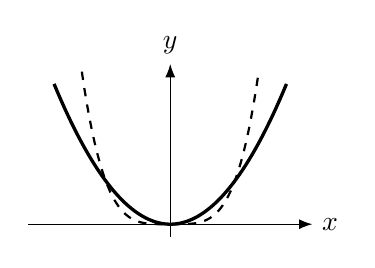
\begin{tikzpicture}[x=.82cm,y=.55cm,>=Latex]
\draw[->](-2.2,0)--(2.2,0)node[right]{$x$};\draw[->](0,-.3)--(0,3.7)node[above]{$y$};
\draw[very thick,domain=-1.8:1.8,samples=70]plot(\x,{\x*\x});
\draw[thick,dashed,domain=-1.37:1.37,samples=70]plot(\x,{\x*\x*\x*\x});
\end{tikzpicture}\par\footnotesize sudé: $x^2$ (plně), $x^4$ (čárkovaně)
\end{minipage}\hfill
\begin{minipage}{.47\linewidth}\centering
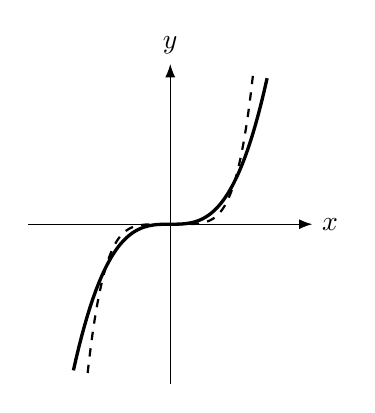
\begin{tikzpicture}[x=.82cm,y=.55cm,>=Latex]
\draw[->](-2.2,0)--(2.2,0)node[right]{$x$};\draw[->](0,-3.7)--(0,3.7)node[above]{$y$};
\draw[very thick,domain=-1.5:1.5,samples=70]plot(\x,{\x*\x*\x});
\draw[thick,dashed,domain=-1.28:1.28,samples=70]plot(\x,{\x*\x*\x*\x*\x});
\end{tikzpicture}\par\footnotesize liché: $x^3$ (plně), $x^5$ (čárkovaně)
\end{minipage}
\end{center}
\poznamka{Grafy jsou ilustrativní výřezy; funkce pokračují dál. Z porovnání v okolí nuly ukaž, že vyšší mocniny v intervalu $(0;1)$ hodnoty zmenšují, kdežto pro $x>1$ je zvětšují.}

\begin{zadaniBox}[title={Věta - Vlastnosti sudých mocnin}]
Je-li $n\ge2$ sudé, potom $f(x)=x^n$ má $D(f)=\mathbb R$, $H(f)=\langle0;+\infty)$, je sudá a na $(-\infty;0\rangle$ klesá, zatímco na $\langle0;+\infty)$ roste. Minimum $0$ má v $x=0$.
\end{zadaniBox}
\noindent\textbf{Zdůvodnění.}\enspace Platí $(-x)^n=x^n\ge0$. Pro větší $|x|$ je $|x|^n$ větší; na záporné poloose se při růstu $x$ absolutní hodnota zmenšuje, na kladné se zvětšuje.


\begin{zadaniBox}[title={Věta - Vlastnosti lichých mocnin}]
Je-li $n\ge1$ liché, potom $f(x)=x^n$ má $D(f)=H(f)=\mathbb R$, je lichá a na celé $\mathbb R$ přísně roste, tedy je i prostá.
\end{zadaniBox}
\noindent\textbf{Zdůvodnění.}\enspace Platí $(-x)^n=-x^n$ a pro $x_1<x_2$ také $x_1^n<x_2^n$; mocnění lichým kladným exponentem zachovává pořadí reálných čísel.


\begin{prikladReseniBox}[title={Příklad 1}]
Porovnej $f(x)=x^4$ a $g(x)=x^5$: sudost/lichost, monotónnost, obor hodnot a prostotu na $\mathbb R$.
\tcblower
$x^4$ je sudá, má $H(f)=\langle0;+\infty)$, klesá na záporné a roste na kladné poloose; na $\mathbb R$ prostá není, neboť $f(-1)=f(1)$. Funkce $x^5$ je lichá, přísně roste na $\mathbb R$, má $H(g)=\mathbb R$ a je prostá.
\end{prikladReseniBox}

\begin{prikladReseniBox}[title={Příklad 2}]
Rozhodni, která z hodnot $\left(\frac{1}{2}\right)^2$, $\left(\frac{1}{2}\right)^4$, $2^2$ a $2^4$ je větší v každé dvojici se stejným základem.
\tcblower
$\left(\frac{1}{2}\right)^2=\frac{1}{4}>\frac{1}{16}=\left(\frac{1}{2}\right)^4$, zatímco $2^2=4<16=2^4$. Účinek zvýšení exponentu závisí na velikosti kladného základu vzhledem k $1$.
\end{prikladReseniBox}

\blok{Samostatná práce}
\begin{zadaniReseniBox}[title={Samostatná práce 1}]
Pro funkce $u(x)=x^6$ a $v(x)=x^7$ urči $D$, $H$, sudost/lichost, prostotu na $\mathbb R$ a znaménko pro $x<0$.
\tcblower
$u$: $D=\mathbb R$, $H=\langle0;+\infty)$, sudá, neprostá, pro záporná nenulová $x$ je kladná. $v$: $D=H=\mathbb R$, lichá, prostá, pro $x<0$ záporná.
\end{zadaniReseniBox}

\begin{zadaniReseniBox}[title={Rozšíření 1}]
Vysvětli, proč je $x^4$ na $\langle0;+\infty)$ prostá, ale na $\mathbb R$ nikoli. Jaký je její inverzní předpis na nezáporném oboru?
\tcblower
Na nezáporných argumentech přísně roste, na celé ose mají $x$ a $-x$ stejný obraz. Pro $D(f)=\langle0;+\infty)$:
\[
\begin{aligned}
f(x)&=x^4 &&\bigm|\ x\to y\\
x&=y^4\\
y&=\sqrt[4]{x}\\
f^{-1}(x)&=\sqrt[4]{x}.
\end{aligned}
\]
$D(f^{-1})=\langle0;+\infty)$.
\end{zadaniReseniBox}

\begin{zadaniReseniBox}[title={Domácí úkol}]
\textbf{Lineární funkce} (od jednodušší k obtížnější):
\begin{enumerate}[label=\alph*)]
\item Urči inverzi k $f(x)=2x+3$ a definiční obor i obor hodnot obou funkcí.
\item Urči inverzi k $g(x)=\frac{3-2x}{4}$ a proveď zkoušku složením.
\end{enumerate}
\textbf{Lineárně lomené funkce}:
\begin{enumerate}[label=\alph*),start=3]
\item Urči inverzi k $h(x)=\frac{2}{x-1}$, obory obou funkcí a jejich asymptoty.
\item Urči inverzi k $k(x)=\frac{2x+3}{x-4}$, obory obou funkcí a jejich asymptoty.
\end{enumerate}
\textbf{Kvadratické funkce}:
\begin{enumerate}[label=\alph*),start=5]
\item Urči inverzi k $m(x)=x^2$ na $D(m)=\langle0;+\infty)$.
\item Urči inverzi k $n(x)=(x-2)^2+1$ na $D(n)=(-\infty;2\rangle$ a její definiční obor.
\end{enumerate}
\textbf{Mocninné funkce}:
\begin{enumerate}[label=\alph*),start=7]
\item Urči $D$, $H$, paritu, monotónnost a prostotu funkce $u(x)=x^4$ na $\mathbb R$.
\item Urči $D$, $H$, paritu, monotónnost a prostotu funkce $v(x)=-2x^3$ na $\mathbb R$; navíc vypočti její inverzi.
\end{enumerate}
\textbf{Znalostní otázky}:
\begin{enumerate}[label=\alph*),start=9]
\item Jaký je rozdíl mezi $f^{-1}(x)$ a $\frac{1}{f(x)}$? Vysvětli na konkrétní funkci.
\item Proč nemá $f(x)=x^2$ na celé $\mathbb R$ inverzní funkci? Jaká dvě omezení jejího oboru vedou ke dvěma různým inverzím?
\end{enumerate}
\tcblower
\begin{enumerate}[label=\alph*)]
\item
\(\displaystyle\begin{aligned}f(x)&=2x+3 &&\bigm|\ x\to y\\x&=2y+3\\2y&=x-3\\y&=\frac{x-3}{2}\\f^{-1}(x)&=\frac{x-3}{2}\end{aligned}\)

Obě funkce mají definiční obor i obor hodnot $\mathbb R$.
\item
\(\displaystyle\begin{aligned}g(x)&=\frac{3-2x}{4} &&\bigm|\ x\to y\\x&=\frac{3-2y}{4}\\4x&=3-2y\\2y&=3-4x\\y&=\frac{3-4x}{2}\\g^{-1}(x)&=\frac{3-4x}{2}\end{aligned}\)

$g(g^{-1}(x))=\frac{3-2\cdot\frac{3-4x}{2}}{4}=x$.
\item
\(\displaystyle\begin{aligned}h(x)&=\frac{2}{x-1} &&\bigm|\ x\to y\\x&=\frac{2}{y-1}\\x(y-1)&=2\\y-1&=\frac{2}{x}\\y&=1+\frac{2}{x}\\h^{-1}(x)&=1+\frac{2}{x}\end{aligned}\)

$D(h)=\mathbb R\setminus\{1\}$, $H(h)=\mathbb R\setminus\{0\}$; $D(h^{-1})=\mathbb R\setminus\{0\}$, $H(h^{-1})=\mathbb R\setminus\{1\}$. Asymptoty $h$: $x=1$, $y=0$; u inverze $x=0$, $y=1$.
\item
\(\displaystyle\begin{aligned}k(x)&=\frac{2x+3}{x-4} &&\bigm|\ x\to y\\x&=\frac{2y+3}{y-4}\\x(y-4)&=2y+3\\xy-4x&=2y+3\\y(x-2)&=4x+3\\y&=\frac{4x+3}{x-2}\\k^{-1}(x)&=\frac{4x+3}{x-2}\end{aligned}\)

$D(k)=\mathbb R\setminus\{4\}$, $H(k)=\mathbb R\setminus\{2\}$; $D(k^{-1})=\mathbb R\setminus\{2\}$, $H(k^{-1})=\mathbb R\setminus\{4\}$. Asymptoty $k$: $x=4$, $y=2$; u inverze $x=2$, $y=4$.
\item
\(\displaystyle\begin{aligned}m(x)&=x^2 &&\bigm|\ x\to y\\x&=y^2\\y&=\sqrt{x}\\m^{-1}(x)&=\sqrt{x}\end{aligned}\)

$D(m^{-1})=H(m^{-1})=\langle0;+\infty)$.
\item
\(\displaystyle\begin{aligned}n(x)&=(x-2)^2+1 &&\bigm|\ x\to y\\x&=(y-2)^2+1\\x-1&=(y-2)^2\\y-2&=-\sqrt{x-1}\\y&=2-\sqrt{x-1}\\n^{-1}(x)&=2-\sqrt{x-1}\end{aligned}\)

$D(n^{-1})=\langle1;+\infty)$, $H(n^{-1})=(-\infty;2\rangle$. Zápornou větev odmocniny určuje $y\le2$.
\item $D(u)=\mathbb R$, $H(u)=\langle0;+\infty)$; $u$ je sudá, klesá na $(-\infty;0\rangle$ a roste na $\langle0;+\infty)$. Na celé $\mathbb R$ není prostá.
\item $D(v)=H(v)=\mathbb R$; funkce je lichá, přísně klesá, a tedy je prostá.

\(\displaystyle\begin{aligned}v(x)&=-2x^3 &&\bigm|\ x\to y\\x&=-2y^3\\y^3&=-\frac{x}{2}\\y&=\sqrt[3]{-\frac{x}{2}}\\v^{-1}(x)&=\sqrt[3]{-\frac{x}{2}}\end{aligned}\)
\item Inverzní funkce vrací původní argument, převrácená hodnota převrací číslo $f(x)$. Například pro $f(x)=2x$ je $f^{-1}(x)=\frac{x}{2}$, kdežto $\frac{1}{f(x)}=\frac{1}{2x}$ (pro $x\ne0$).
\item Protože $f(-2)=f(2)=4$, není na $\mathbb R$ prostá. Při omezení na $\langle0;+\infty)$ je inverze $\sqrt{x}$, při omezení na $(-\infty;0\rangle$ je inverze $-\sqrt{x}$, obě s definičním oborem $\langle0;+\infty)$.
\end{enumerate}
\end{zadaniReseniBox}
\end{document}
